\documentclass{beamer}
\usepackage{graphics}
\title{An introduction to the AHIR-v2 tool-set}
\author{Madhav P. Desai\\ Department of Electrical Engg.\\ IIT Bombay, Mumbai India}
\date{March 8, 2018}
\begin{document}
\maketitle



\frame[containsverbatim]{\frametitle{The purpose of the toolset}

\begin{itemize}
\item Aid in the design and implementation of complex systems (in hardware).
\item Describe the algorithm (behaviour) of the system using high-level
languages, and migrate the algorithm to a hardware
implementation.
\begin{itemize}
\item C.
\item Aa.
\end{itemize}
\end{itemize}
}

\frame[containsverbatim]{\frametitle{Plan}
\begin{itemize}
\item Introduction: going from C to VHDL and simulating the VHDL.
\begin{itemize}
\item Exercise: go through a couple of examples.
\end{itemize}
\item Understand the hardware target model used by the AHIR-V2 tools.
\begin{itemize}
\item Exercise: re-visit the examples to take a closer look.
\end{itemize}
\item Optimizations.
\item Loop-pipelining.
\item {\bf Aa} language.
\item Design problem.
\begin{itemize}
\item Design a programmable FIR filter.
\end{itemize}
\end{itemize}
}


\frame[containsverbatim]{\frametitle{For example}

Design a circuit that takes two inputs, computes the maximum of
the two and returns the maximum.
\begin{verbatim}
uint32_t maxOfTwo(uint32_t a, uint32_t b)
{
  uint32_t c = ((a > b) ? a : b);
}
\end{verbatim}
}


\frame[containsverbatim]{\frametitle{Lets write a test-program to check this code}
\begin{verbatim}
uint32_t maxOfTwo(uint32_t, uint32_t);
int main(int argc, char* argv[])
{
  if(argc < 3)
  {
     printf(stderr, "%s <uint32_t> <uint32_t>\n", argv[0]);
     return(1);
  }
  uint32_t c = maxOfTwo(atoi(argv[1]), atoi(argv[2]));
  printf(stdout,"Result = %d.\n", c);
  return(0);
}
\end{verbatim}
}

\frame[containsverbatim]{\frametitle{We compile and run it}

Go to ex1/ and check it out.

}

\frame[containsverbatim]{\frametitle{AHIR flow}
\begin{figure}
  \centering
  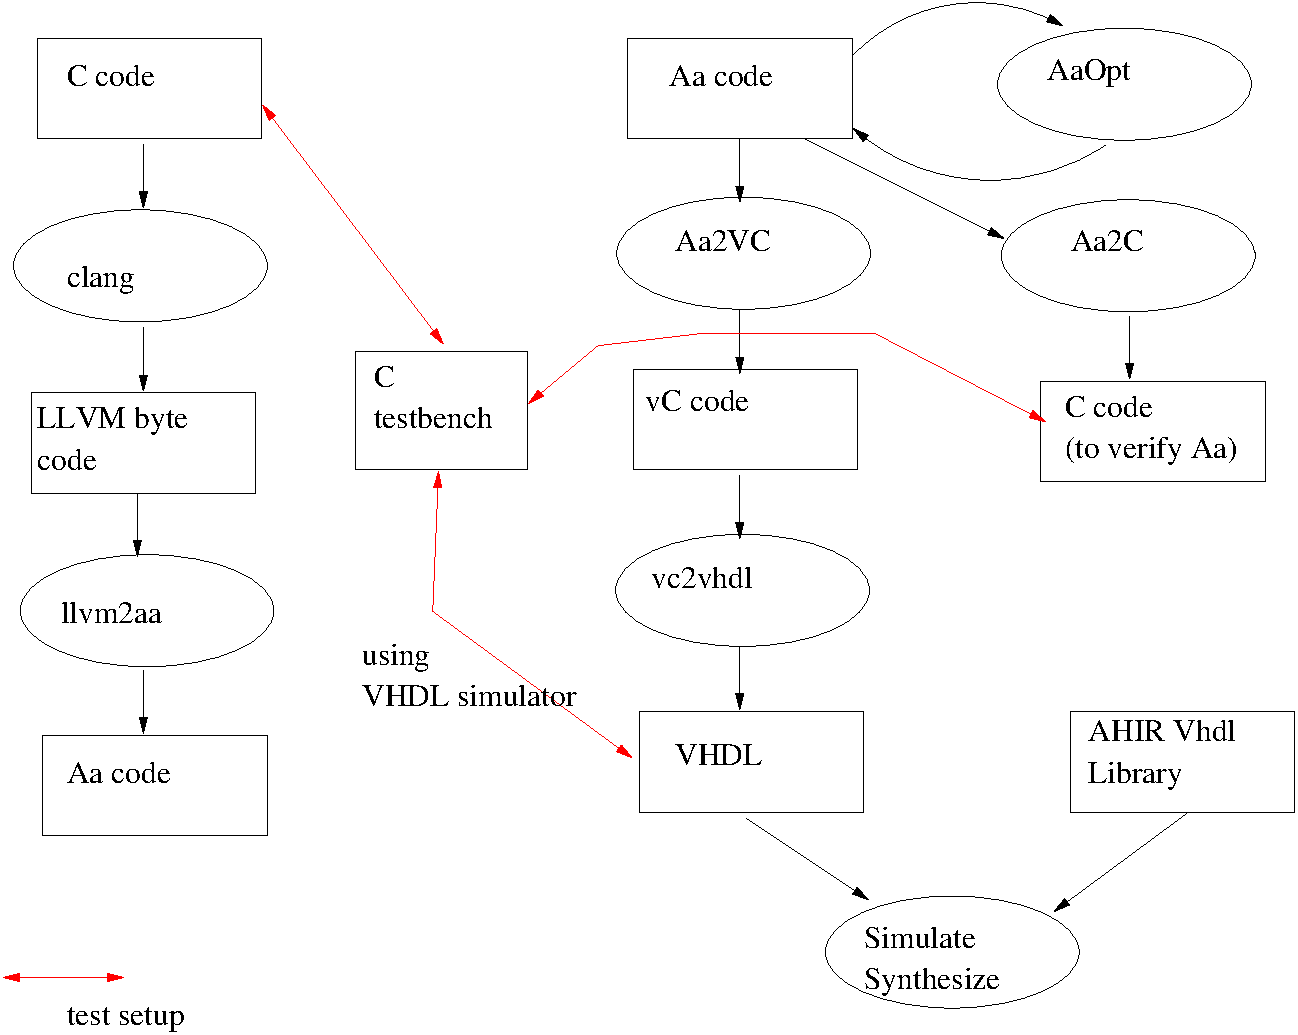
\includegraphics[width=10cm]{figs/AhirFlow.pdf}
  \caption{AHIR flow}
\end{figure}
}


\frame[containsverbatim]{\frametitle{Conversion to hardware}

The AHIR-v2 flow translates the code to hardware in four steps:
\begin{enumerate}
\item The source C code is compiled using the open-source compiler
{\bf clang} (we use version 2.8), which produces byte-code in {\bf llvm}
format.
\item We take the {\bf llvm} bytecode and translate it to our internal
representation called {\bf Aa}.  This is done by a utility called {\bf llvm2aa}.
\item Multiple {\bf Aa} files can be linked using an {\bf Aa} linker
tool called {\bf AaLinkExtMem}.
\item The linked {\bf Aa} code is then converted to a virtual circuit using
a {\bf vC} representation.  This is done using a utility called {\bf aa2vc}.
\item Finally, the {\bf vC} code is converted to VHDL which can then
be simulated or synthesized.  This conversion is done using a utility
called {\bf vc2vhdl}.
\end{enumerate}
At each stage, various optimizations are carried out.
}

\frame[containsverbatim]{\frametitle{Lets see what happens}

Go back to ex1/ and check it out.

}

\frame[containsverbatim]{\frametitle{VHDL Structure}
\begin{figure}
  \centering
  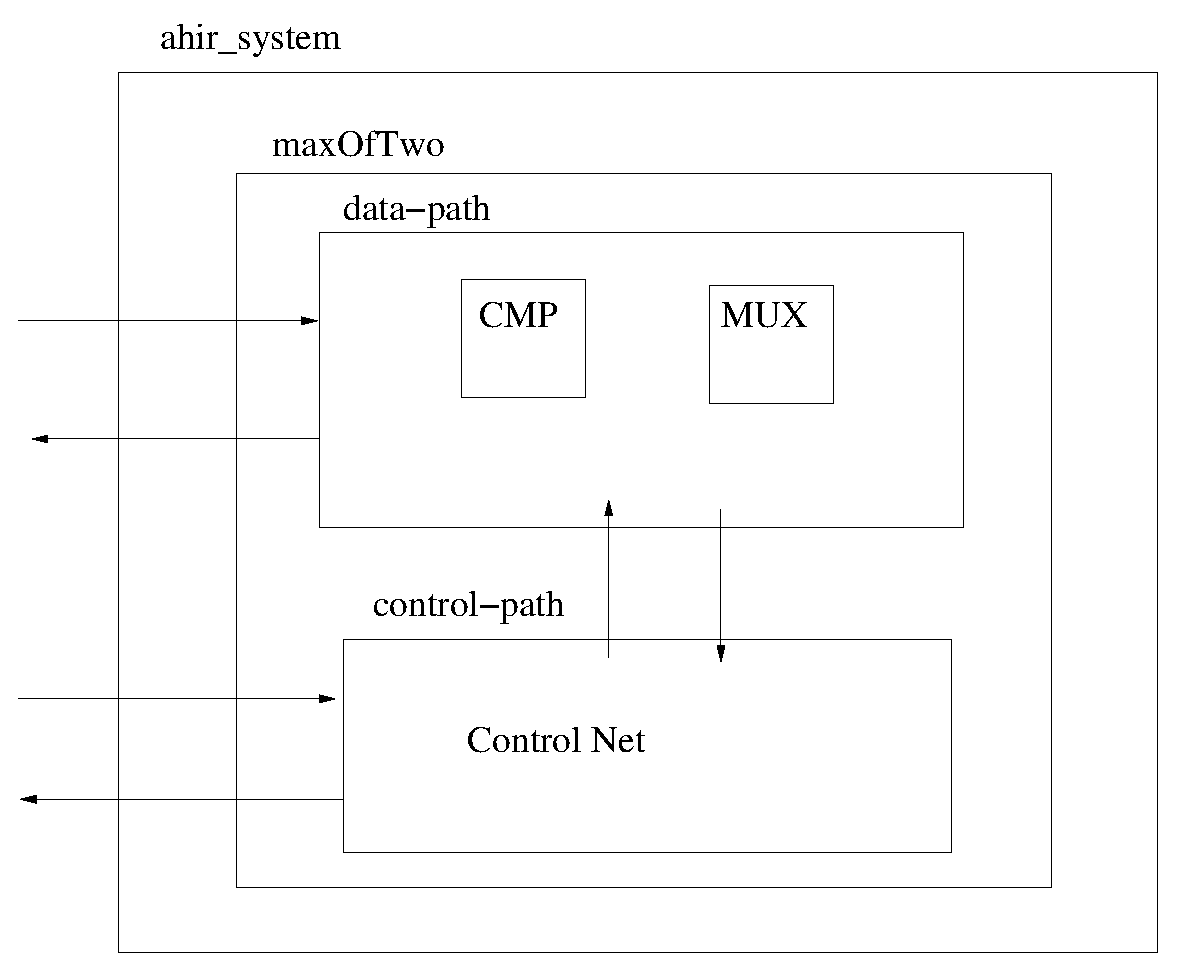
\includegraphics[width=10cm]{ex1/figs/VhdlStructure.eps}
  \caption{VHDL structure of generated example}
\end{figure}
}


\frame[containsverbatim]{\frametitle{Validating the VHDL}

\begin{itemize}
\item In order to test the VHDL, we will use the same program
that was used to test the original C code.
\item Two processes are started: one executing the test-program
and the other executing a VHDL simulator which simulates the
generated VHDL.  The two processes communicate through sockets.
\item There is no need to write a new test-bench!
\end{itemize}
}


\frame[containsverbatim]{\frametitle{Lets take a look}
Go back to ex1/ and check it out.
}

\frame[containsverbatim]{\frametitle{Lets make it a  little more interesting}
\begin{verbatim}
float x_vals[2];
void firDaemon()
{
  x_vals[0] = 0.0; x_vals[1] = 0.0;
  uint8_t head_pointer = 0;
  // fir loop.
  while(1)
  {
    float x = read_float32("in_data");
    float y = 0.8*x + (0.15*x_vals[head_pointer]) + 
                (0.05*x_vals[(head_pointer+1)&0x1]);
    write_float32("out_data",y);
    head_pointer = (head_pointer + 1)&0x1;
    x_vals[head_pointer] = x;
  }
}
\end{verbatim}
}

\frame[containsverbatim]{\frametitle{The testbench for the Daemon}
\begin{verbatim}
int main(int argc, char* argv[])
{
  while(1)
  {
    float a;
    scanf("%f", &a);
    write_float32("in_data",a);
    float c = read_float32("out_data");
    fprintf(stdout,"Result = %f.\n", c);
  }
  return(0);
}
\end{verbatim}
}


\frame[containsverbatim]{\frametitle{The testbench for the Daemon}
Lets check out the software and the hardware generated from it. 
Go to ex2/.
}


\frame[containsverbatim]{\frametitle{Download and Install}
\begin{itemize}
\item Clone git repository
\begin{verbatim}
git clone https://github.com/madhavPdesai/ahir.git .
\end{verbatim}
\item Install llvm-2.8, clang-2.8 from www.llvm.org (from source, builds on ubuntu 12, centos 6.5, may need  to do minor edits in includes in ubuntu 14).
\item Install boost development packages.
\item Install antlr-2.7.7 (from source, builds on ubuntu 12, centos 6.5, some includes need to be added in ubuntu 14).
\item Install java run-time (openjdk).
\item Install ghdl (or modelsim).
\item Go to release directory. 
\begin{verbatim}
source ahir_bashrc
mkdir bin
./build.sh
\end{verbatim}
\item Should work..
\end{itemize}
}

\end{document}
